\documentclass[12pt]{article}
\usepackage[utf8]{inputenc}
\usepackage{amsmath}
\usepackage{amssymb}
\usepackage{graphics}
\usepackage{graphicx}
\usepackage{array}
\usepackage{hyperref}
\usepackage{xcolor}
\usepackage{float}
\usepackage[french]{babel}
\usepackage[T1]{fontenc}
\usepackage[a4paper, total={6.5in, 10in}]{geometry}

\begin{document}
\begin{titlepage}
	\centering
	
	
	\vspace{0.5cm}
	{\Large \scshape\bfseries KT IT responsible}
	\vspace{0.5cm}

	{ \Huge }
	

	{\itshape V2023.1 \large  Jacques HOGGE \par}
	{\itshape V2023.2 \large  Jacques HOGGE \par}
	{\itshape V2024.1 \large  Guillaume Dupont \par}

	\vspace{5cm}
	
	
	\textit{Il s'agit d'une reformulation du KT d'avant car on a du changer de site et donc tous n'est plus trop a jour (bis)}
	

	\vfill
	
    {\Large  \today}
\end{titlepage}
\newpage

\section{GoogleSites}\label{GoogleSites}
	Notre site est géré et hébergé par GoogleSites et nous avons les noms de domaines avec OVH.
	
	\subsection{Accès au site}
		Pour accéder au site, tu dois juste te rendre sur le drive de l'addresse mail IT. Dans ce drive se trouve le site et tous les documents (images, pdf, ...) qui se trouvent sur le site.
	 	\begin{figure}[htp]
			\centering
			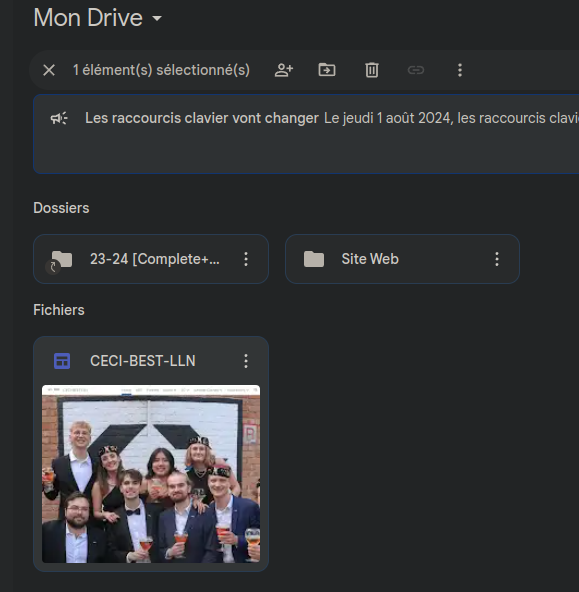
\includegraphics[width=0.6\textwidth]{img/AccessSite.png}
		\end{figure} 

	 \subsection{Évènements}
	 	Il faudra a certain moment crée une nouvelle page afin de parler d'un évènement que l'on organise (EC (RIP EBEC), Hackathon, Summer ...). Normalement c'est les MO (ou responsable du poste) de l'event qui est responsable de rédiger l'article a mettre sur la page.Il faut donc pas hésiter a les SPAM comme des porc afin d'avoir l'article a temps. Je vous conseille de poser un DL sinon il ne va jamais vous faire ton article car il est "occupé a autre chose".
	 	
	 	Bien que il y a Facebook, Insta, Onlyfans pour faire la pub de nos events et que le site est un peu obsolète, celui-ci sert principalement d'archive de CECI-BEST. Il faut cependant quand meme faire l'article car celui-ci permet un visuel pour nos sponsors.
	 	
	 	Pour faire une page, il suffit de copier une page déja faite et changer le titre, les photos, le texte, les responsable et ajouter des boutons qui ramène vers le formulaire d'inscription et/ou a l'event Facebook.
	\newpage
	 \subsection{Créer une page}
	 	Rien de très sorcier, il suffit d'aller en bas à droite sur le petit menu +.
	 	\begin{figure}[htp]
			\centering
			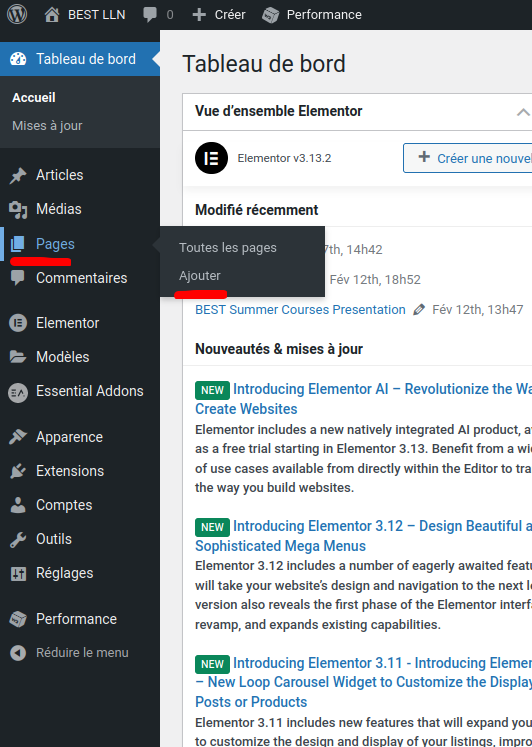
\includegraphics[width=0.6\textwidth]{img/CreerPage.png}
		\end{figure}
		
		Pour garder de jolies URL, il faut masquer la page de la navigation.
		\begin{figure}[htp]
			\centering
			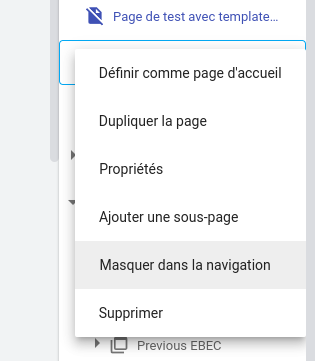
\includegraphics[width=0.6\textwidth]{img/Mask.png}
		\end{figure}

		Ensuite tu cliques sur la section où tu veux mettre la page et tu vas rajouter un lien comme si tu faisais une nouvelle page.

		Pour remplir la page inspire toi des précédents articles pour garder une certaine cohérence sur le site.
		
	\subsection{Editer une page}
		Encore moins compliqué qu'en créer une. Tu cliques juste sur la page que tu veux modifier et puis tu veux ce que tu veux.
		
	\subsection{Sponsors}
			
	Il est obligatoire de tenir notre pages des sponsors a jour, c'est dans le contrat que on leur donneras de la visibilité donc si on le fait pas on est dans la merde.
	Pour se faire, il suffit de demander au FR quelle sponsors doivent etres mis sur le site et avec quelle photo et texte. Il ne faut pas hesiter a obliger les photos et le texte au FR car peut etre que les entreprises on des exigences particulière. Ou alors vous pouvez aller voire dans le drive du FR, si celui-ci est doué, tous est la.
	Attention certain sponsors sont a l'année alors que d'autre sont peut etre juste pour un événement, a toi de demander et savoir mettre en jour en fonction de cela. 
	Tu peux juste dupliquer une des précédentes sections et changer avec la photo et le texte que tu as reçu.	
	En plus de la page sponsors, il faut aussi les ajouter sur la page  de l'event et sur la page d'accueil.Pour la page d'accueil tu peux le mettre dans le peit carousel avec les autres sponsors et pour l'event, tu rajoutes une petite photo. Dans les deux cas mets un petit lien qui redirige vers la page des sponsors.
	
	\subsection{Nouveaux et Anciens Board}
	Une fois les photos de l'ouverture reçues, tu peux mettre à jour la page du Board actuel avec la photo de groupe et individuelles.
	Plus un blague que un point réel mais les anciens veulent le moment de gloire et oblige que ils soient présent sur la page des anciens Board avec l'année du board et le Nom de celui-ci avec chaque photo et leur poste.
	Pour t'aider j'ai créer une page template dont tu peux copier la section pour remplir sur la page avec les anciens Board.
	\begin{figure}[htp]
		\centering
		
\includegraphics[width=0.6\textwidth]{img/TemplateBoard.png}
	\end{figure} 
	
	
\section{OVH}
	OVH est notre hebergeur pour le site\footnote{On espère que le serveur ne brulera pas} et qui attribue les domaines \textit{www.best-lln.eu} et \textit{www.best-lln.be}\footnote{C'est le nom de domaine de l'ancien site, on a garder le nom de domaine et fait une redirection vers le nouveau site, ça coute pas trop cher donc a voir avec la trésoreries si vous le laisser ou pas}. 
	\subsection{Creer un sauvegarde}
	\label{creersauvegarde}
		Pour ce faire, il faut se connecter au compte OVH, se rendre sur l'hébergement \textit{best.lln.eu}
		
		\begin{figure}[htp]
			\centering
			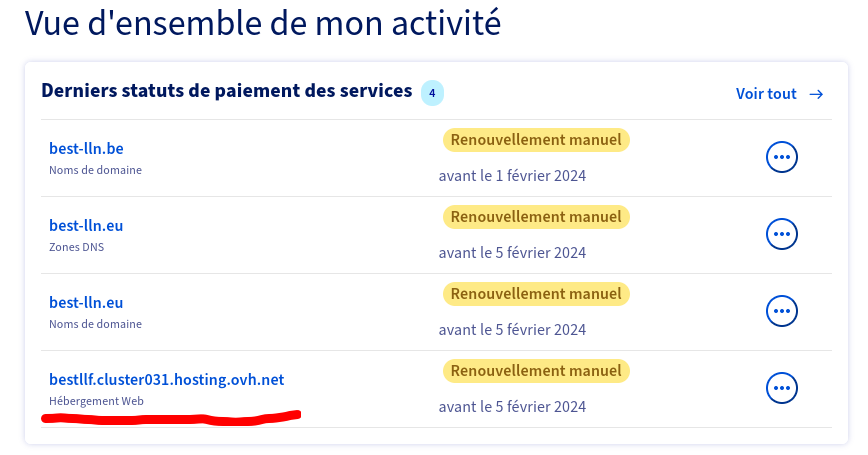
\includegraphics[width=0.5\textwidth]{img/OVH.png}
		\end{figure}
		
		\vfill
		
		\begin{figure}[htp]
			\centering
			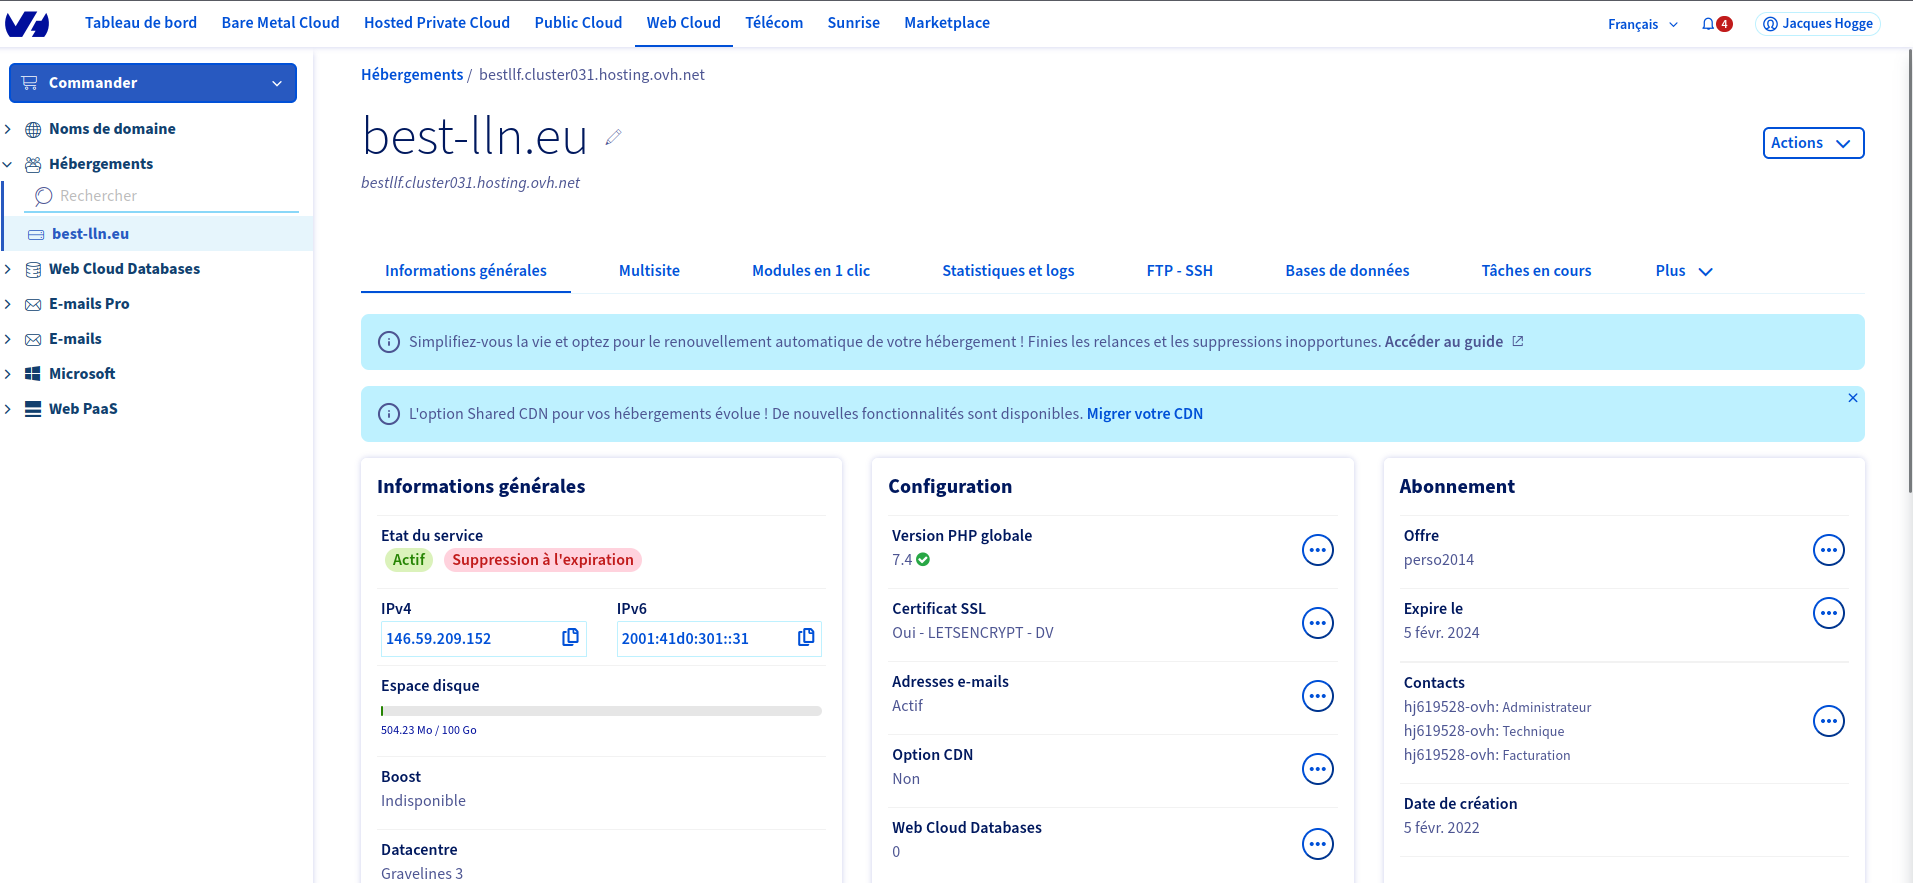
\includegraphics[width=.8\textwidth]{img/OVH1.png}
		\end{figure}
		
		Il y a plein de fonctionnalité que vous pouvez découvrir, ne faite pas trop de betise cela-dit. Pour la sauvegarde, il faut aller dans Bases de données. Une fois la dedans, il suffit de cliquer sur les 3 points et faire "Creer une sauvegarde" et choisir la date d'aujourdhui.
		
		Pour l'instant il y a encore de la place pour pas mal de sauvegarde mais au fil du temps hesiter pas a retirer les trop ancienne. Et si vous vous chauffer vous pouvez mettre les anciennes sauvegarde dans la \textit{Wayback machine}\footnote{\url{https://archive.org/web/}} et ainsi voir dans le futur a quoi ressemblait le site avant.
		
		\begin{figure}[htp]
			\centering
			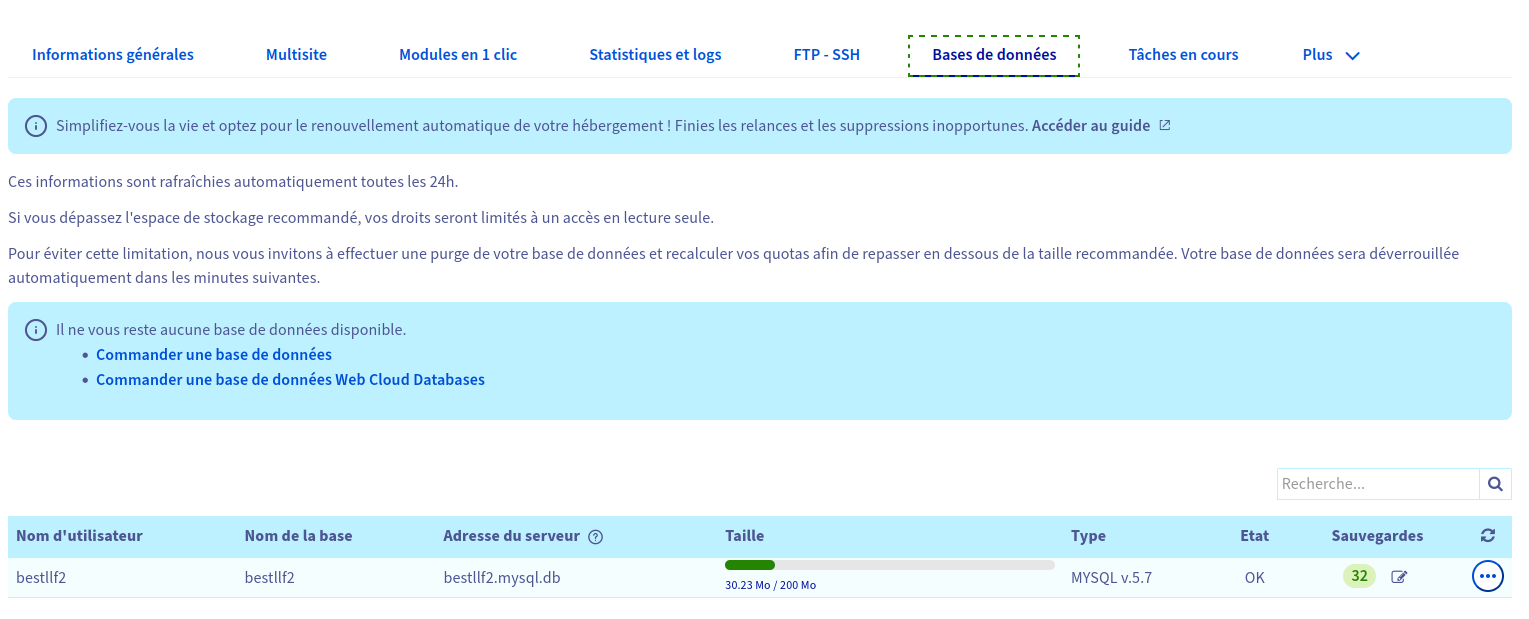
\includegraphics[width=.8\textwidth]{img/OVH2.png}
		\end{figure}
		
	
	\subsection{Récupérer une sauvegarde du site}
		Si jamais tu as fait une connerie, ou que tu veux revenir en arrière, il suffit de faire comment dans la \autoref{creersauvegarde} mais au lieu de créer un nouvelle sauvegarde, il faut \textit{Restaurer une sauvegarde} et voila.
		
	\subsection{Redirection}
		Il y a une redirection qui est faite avec le nom de domaine \textit{www.best-lln.be}. Il suffit d'aller dans le menu a gauche dans Noms de domaine $\rightarrow$ best-lln.be $\rightarrow$ Redirection. et la tu voix toutes les redirection, la plus part sont en lien avec le DNS ou les CNAME donc ne t'en occupe pas. Tu peux en ajouter une nouvelle avec \textit{Ajouter une redirection} a droite.
		
	\subsection{Autre}
		Il y a plein d'autre fonctionnalité sur OVH tels que voire le trafic sur le site etc. Hesite pas a visiter et google les ton amis et les anciens IT aussi
		
\section{Github}
	Depuis 2023 le CECI-BEST possède une github qui est nécessaire pour les Hackhaton qui sont organisé. La responsabilité est techniquement celle de l'IT qui devra aller voire les différent groupes afin de s'ajouter sur le git et garder ainsi une archive. Vous pouvrez aussi les télécharger si vous avez peur que il vont disparetre
	
	les identifiant sont sur le drive et sinon vous pouvez demander a un ancien IT ou a la PR qui normalement doit les connaitres.

	Sur le github, il y a moyen des créer des "dossier" qui comporte different repo github. il suffit d'en créer un par année et de rajouter les repos dedans. Cela est possible avec le syteme "favoris".
	
	Google est ton amis et regarde comment c'est fait avant.
	
\section{Changement proprio Wordpress}
	A faire avec l'ancien IT
	\begin{enumerate}
		\item Ancien IT ajoute le nouveau IT dans les responsable du Wordpress via l’onglet Utilisateurs de l’interface Wordpress

		\item Le nouveau IT donne quand a lui sont adresse mail et sont identifiant
	\end{enumerate}
	

\section{Changement proprio OVH}
	\begin{enumerate}
		\item Le nouvel IT se crée un compte avec son adresse perso (ou BEST comme il veut)
		\item le nouvel IT donne sont identifiant a l'ancien IT (truc du genre aa123456-ovh)
		\item L’ancien gestionnaire change les contacts pour l’hébergement, emails, zone dns et domaine dans son espace OVH (Plus > Gérer les contacts)
		\item Confirmation par mail des 2 coté
	\end{enumerate}
	
\section{Hacked}	
	Il est déja arrivé plusieur fois que on se soit fait Hacker. On parle plus d'un malware qui redirige notre site vers un site de scam. Souvent c'est parceque une script Js a été ajouté dans le header, il font donc le retrouver et le retirer.

Le plus souvent les raisons de ce problèmes  ne sont pas de vous mais de Wordpress et plus particulièrement Elementor qui laisse des breches de sécurité et qui permet au hacker de se connecter au compte. Il faut donc bien faire attention durant les grosse mise-a-jour et voire les différente modification. Et aussi peut etre un peu attendre avant pour voir si il font pas des mise-a-jour de la sécurité juste apres.
	
	Verifier aussi de temps-en-temps si des comptes ne se sont pas rajouter, si c'est le cas, changer tous de suite les mots-de-passe. Ajouter aussi une authentification a double facteur.
	
\section{PHP}
	Notre site est sous PHP avec wordpress, le soucis est que c'est voué a disparaitre, PHP n'est plus aussi sécurisé et utile que avant. Donc petit conseille de ma part. Continuer de garder, et si un jour celui-ci est mort, ne refaite pas un Wordpresse et passer a autre chose. Il est peut etre possible d'utiliser Odoo gratuitement et même avoir un partenaria avec eu justement.



\section{Poste}

	IT est un poste qui selon certaines personnes ne sert a rien ou ne travaille pas. Peut importe ce que tu dit il diront que tu ne fais rien et cela est normal car ce que tu fais n'est pas directement visible
	
	Donc faut pas le prendre mal quand il disent que tu fais riens.
	\subsection{Slides}
	
	l'IT est aussi responsable du rétroprojecteur qui est au local et qu'il faut prendre pour afficher les slides au réunions. rien de tres sorcier il suffit de demander au gens de mettre les slides dans ton fichiers du drives
	
	\subsection{Wooclap}
		Lors de gros vote important (proposale, membership ...) vous utiliserez un wooclap afin d'avoir un systheme de votes pour chaque membre de la réunions. Il suffit de creer un comptes (je conseille d'utiliser l'adresse UCL car tu as le prémium gratuit et donc un nombre illimité de wooclap).
		
	\subsection{Clown}
		L'IT est la personne la plus drole du Board, c'est comme ça c'est la regles, il faut donc tous le temps dires des blagues et faire des bullshit marrant. Attention il faut savoir etre sérieux quand il le faut
	
	\subsection{\textcolor{red}{TRITOUFS}}
		
		La tradition veut que les IT soient des gens expérimentés dans l’art de BWAR. il faut donc se spécialisé dans l’art du Tritouf au fil de mon mandat, c’est pourquoi c’est un plus pour ton poste si tu sais bien en faire (Ca va chier au rachat). 
		
		\begin{enumerate}
			\item Se munir de trois gobelets (réutilisables \#GreenTeam) 
			\item Les remplir généreusement avec de la bière
			\item Les aligner selon ta bonne guise 
			\item Souffler un bon coup 
			\item Boire le premier 
			\item Boire le deuxieme
			\item Boire le troisieme
			\item Éventuellement vomir
			\item Recommencer à partir du point 1. 

		\end{enumerate}
		
		Le but étant bien sûr de vider tous ses verres ENTIÈREMENT. Pas nécessairement le plus vite possible MAIS c’est un plus, naturellement.   


		De nombreuses séances d'apprentissage seront organisées pendant le Summer Course ainsi que des séances d’examen. Bonne chance. 


\section{Conclusion}
	Le post IT c'est le meilleur
		
		
\end{document}